% 请在下方的大括号相应位置填写正确的节标题和标签,以及作者姓名
\section{能带绘图与后处理}\label{sec:能带绘图与后处理}
\sectionAuthor{Jiaqi Z.}

% 请在下方的item内填写本节知识点
\begin{Abstract}
    \item 如何使用Origin绘制能带图
    \item 如何使用vaspkit自动生成能带图
\end{Abstract}

% 请在正文相应位置填写正确的小节标题(或小小节标题),同时将标签的“节标题”和“小节标题”改为实际内容

在上一节的计算中,我们已经得到了能带所需要的全部信息。但是,使用计算软件得到的仅仅是数据,与我们所需要的“\emph{能带图}”还差一个步骤--数据后处理。

在这一节,我们将讨论如何借助于vaspkit软件绘制能带图。其中,最基本的方法是使用Origin绘图,但在vaspkit的更新过程中,也添加了借助于Python脚本自动绘图的功能。我们将在本节首先介绍如何配置可自动绘图的vaspkit,然后介绍如何使用vaspkit自动绘图。

\begin{attention}
    vaspkit自动绘图并不一定在所有版本都可用,同时这依赖于服务器的配置是否有必要的包(如Python,matplotlib等)。因此,你不应当将vaspkit自动绘图作为依赖,而是作为一个“备选项”。

    使用Origin绘图应当是绘制能带图首先需要掌握的内容。
\end{attention}

\subsection{使用Origin绘制能带图}\label{subsec:能带绘图与后处理-使用Origin绘制能带图}

使用Origin绘制能带图的第一步是\emph{得到能带图上每一点的坐标},借助于vaspkit我们可以很容易实现。利用\code{vaspkit-211}可以得到绘制能带图所需要的\code{BAND.dat}文件,其中包含了能带图的数据点坐标,下面则是文件开始的一部分:

\begin{lstlisting}[caption=BAND.dat]
#K-Path(1/A) Energy-Level(eV)
# NKPTS & NBANDS: 180  64
# Band-Index    1
    0.00000    -19.370800
    0.04630    -19.368108
    0.09260    -19.360010
    0.13890    -19.346551
    0.18520    -19.327775
    0.23150    -19.303736
    0.27780    -19.274533
\end{lstlisting}

除此之外,我们还会得到\code{KLINES.dat}文件,用于生成高对称点坐标。将这两个文件下载到本地后,导入Origin软件当中。在\code{BAND.dat}文件后新添一列,并将\code{KLINES.dat}文件复制到新添的列中,得到的文件如图\ref{fig:能带绘图与后处理-BAND.dat修改后}所示。

\begin{figure}
    \centering
    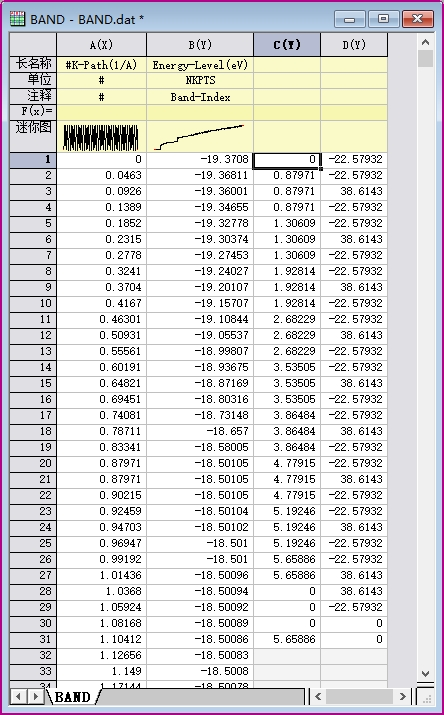
\includegraphics[width=1\linewidth]{VASP计算/能带计算/能带绘图与后处理/fig/BAND_dat.png}
    \caption{\code{BAND.dat}修改后}
    \label{fig:能带绘图与后处理-BAND.dat修改后}
\end{figure}

将新添加的C列(\code{KLINES.dat}文件中的x坐标的属性设置为“X”(方法:右键点击上方列名-“设置为”-X)

将这4列数据全选后点击菜单栏“绘图”-“基础2D图”-“折线图”即可得到所绘制的能带如图\ref{fig:能带绘图与后处理-Origin生成的能带图}所示。

\begin{figure}
    \centering
    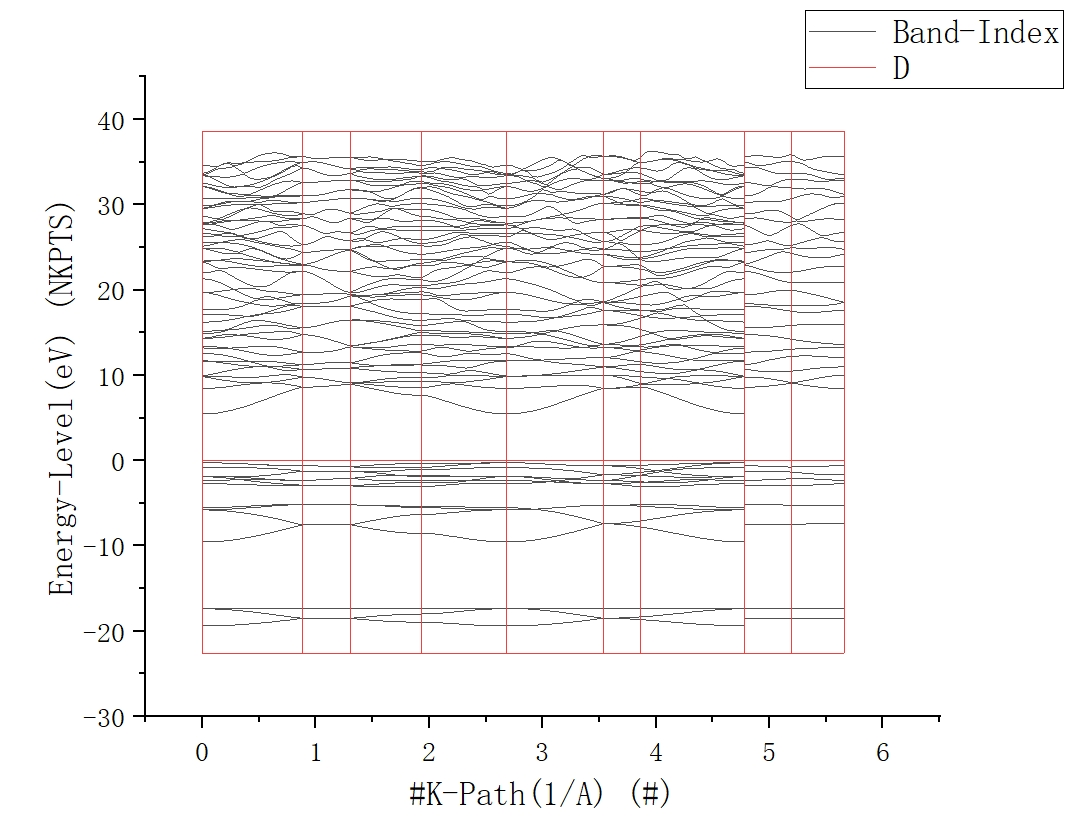
\includegraphics[width=1\linewidth]{VASP计算/能带计算/能带绘图与后处理/fig/Origin生成能带.png}
    \caption{Origin生成的能带图}
    \label{fig:能带绘图与后处理-Origin生成的能带图}
\end{figure}

调整线型与坐标范围,并在下方添加高对称点标签(可以借助于vaspkit生成的\code{KLABELS}文件,其中包含所有高对称点坐标所对应的x轴坐标)

\begin{attention}
    一般来说,默认生成的能带图都会如图\ref{fig:能带绘图与后处理-Origin生成的能带图}所示包含较多的能带。但在实际研究中,我们往往仅关心费米能级附近(即0点附近)的情况。此时除了可以使用Origin调整坐标轴范围的方法,也可以在使用VASP计算自洽和能带的时候使用\code{NBANDS}参数,设置\emph{需要显示的能带数量}。

    在使用vaspkit自动生成能带图时,则需要对这一参数进行设置。
\end{attention}

处理后得到的能带图如图\ref{fig:能带绘图与后处理-SiO2能带图}所示\footnote{绘图配色可以根据自己喜好选择。}

\begin{figure}
    \centering
    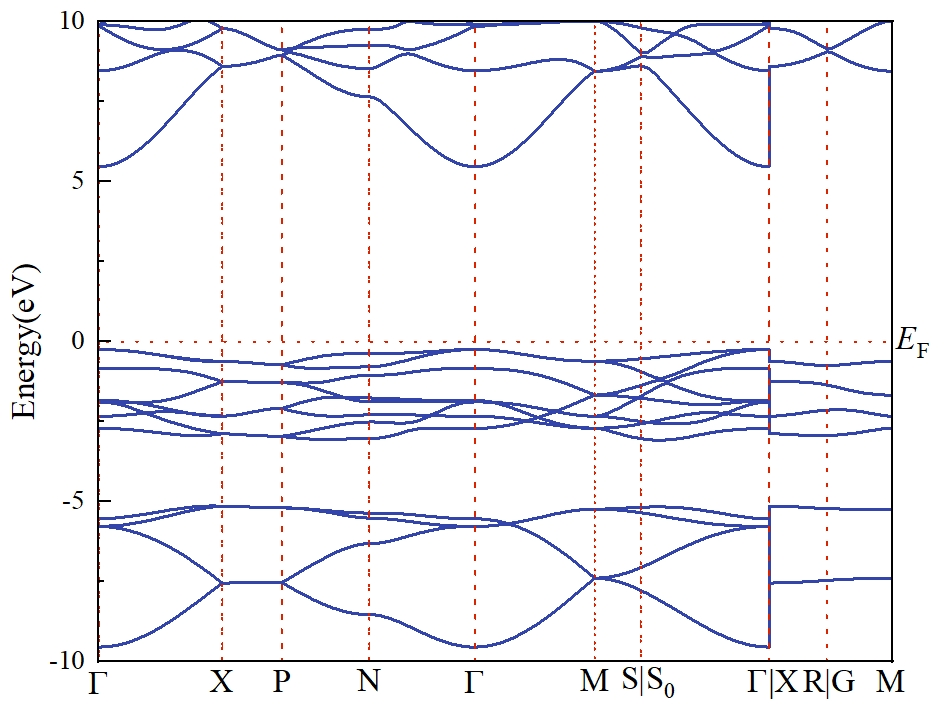
\includegraphics[width=1\linewidth]{VASP计算/能带计算/能带绘图与后处理/fig/SiO2能带图.png}
    \caption{\ch{SiO2}能带图}
    \label{fig:能带绘图与后处理-SiO2能带图}
\end{figure}

\subsection{使用vaspkit自动生成能带图}\label{subsec:能带绘图与后处理-使用vaspkit自动生成能带图}

自1.2.5版本之后,vaspkit更新了自动绘图的功能。利用这一功能,可以不将数据下载至本地后使用Origin绘图,而是直接在Linux操作系统中得到能带图像。

使用vaspkit自动绘图的过程是比较简单的,但我们需要提前对vaspkit做一些配置上的设置。

\subsubsection{vaspkit配置过程}

\begin{attention}
    请首先检查你所使用的vaspkit是否为1.2.5或更新版本。你可以直接使用\code{vaspkit}命令,在菜单栏上方,可以查看所使用的软件版本。

    同时,你还应当确认你的系统上已经配置了Python相关环境,以及绘图所必须的matplotlib包。通常,使用Anaconda可以“一次性”完成Python所需要的所有配置。确认是否安装Anaconda的一个方法是使用命令\code{conda --version},若输出版本号,则表明已经配置了Anaconda\footnote{在有些服务器上,可能需要其他设置引入Anaconda模块。例如,在我所在课题组的服务器上,使用之前需要调用\code{module load anaconda3}导入相关模块。}。

    如果存在没有的命令或模块,可能需要重新安装。详细安装过程请查阅对应软件官网\footnote{VASPKIT官网:https://vaspkit.com/}\footnote{Anaconda官网:https://www.anaconda.com/}的说明。
\end{attention}

假设你的系统已经确认可以配置,在开始之前还需要做如下操作:

\begin{enumerate}
    \item 使用\code{which python3}查看\emph{python3所在目录}。你需要记住这一路径,将其首先复制到本地的记事本或其他地方是一个好方法;
    \item 使用\code{which vaspkit}查看\emph{vaspkit所在目录},并使用\code{cd}命令进入这一目录(通常只需要进入到版本号所在目录即可,例如,在我所在课题组当中,目录为\code{/opt/pub/softwares/VASPKIT/1.5.1});
    \item 在这一目录下,找到\code{how\_to\_set\_environment\_variables}文件,并将其中从\code{\#BEGIN\_CUSTOMIZE\_PLOT}到\code{\#END\_CUSTOMIZE\_PLOT}之间的所有内容(包括这两行)复制到某个地方,以便稍后使用;
    \item 回到所在家目录,新建一个\code{.vaspkit}文件,并在其中创建如下两行:
    \begin{lstlisting}[caption=.vaspkit]
PYTHON_BIN    /opt/pub/toolkits/anaconda3/bin/python3
AUTO_PLOT     .TRUE.
    \end{lstlisting}
    其中,\code{PYTHON\_BIN}后面对应的是之前所复制的python3所在目录。然后,在文件下方将所复制的\code{\#BEGIN\_CUSTOMIZE\_PLOT}到\code{\#END\_CUSTOMIZE\_PLOT}之间的所有内容粘贴至后面。
\end{enumerate}

\subsubsection{使用vaspkit绘图}

在使用vaspkit绘图前,应当首先保证你已经导入了相应模块(如Anaconda等)。与正常使用vaspkit导出能带图类似,在使用\code{vaspkit-211}导出时,会询问导出图片是仅导出能带图,还是能带图加态密度。我们在这里选择仅绘制能带图(1),得到如图所示的图像。

\begin{figure}
    \centering
    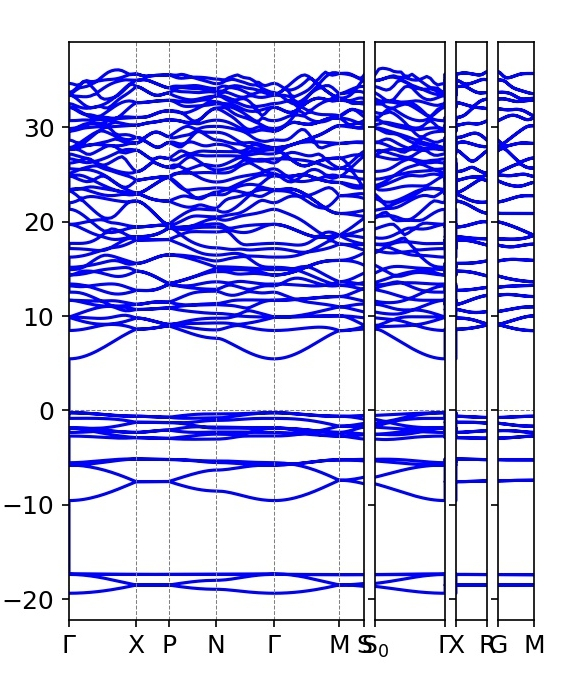
\includegraphics[width=1\linewidth]{VASP计算/能带计算/能带绘图与后处理/fig/vaspkit自动生成能带图.png}
    \caption{使用vaspkit生成能带图}
    \label{fig:使用vaspkit生成能带图}
\end{figure}

\begin{extend}
    正如你所见那样,使用vaspkit默认生成的能带图是很大的能量范围,且不能对其进行调整。一个简单的方法是在计算时使用\keyword{EMIN}和\keyword{EMAX}参数设置能量区间。
\end{extend}

\subsection{如何计算带隙}\label{subsec:能带绘图与后处理-如何计算带隙}

有时,我们可能不是强制要求需要得到能带图,而仅仅关注结构的带隙性质(如带隙大小,类型等)。此时,可以直接使用在绘图过程中生成的\code{BAND\_GAP}文件(使用\code{vaspkit-211}生成)。以\ch{SiO2}为例,文件内容为:

\begin{lstlisting}[caption=BAND\_GAP]
Band Character:    Direct
Band Gap (eV):    5.7105
Eigenvalue of VBM (eV):   -0.6699
Eigenvalue of CBM (eV):    5.0407
Fermi Energy (eV):   -0.4270
HOMO & LUMO Bands:        16        17
Location of VBM: -0.000000  0.000000  0.000000
Location of CBM: -0.000000  0.000000  0.000000
\end{lstlisting}

其中,\code{Band Character}表明带隙类型是直接带隙(Direct)或间接带隙(Inderect);\code{Band Gap}表明所计算结构的带隙大小,在本例中为5.71 eV。除此之外,这一文件还提供了如HOMO(最高占据分子轨道)和LUMO(最低未占据分子轨道)所对应的能带条数,以及VBM(价带顶)和CBM(导带底)所对应的K点坐标。

\begin{attention}
    如果你关注过最开始Materials Project所记录的数据,可能会发现,数据库内所给的带隙约为5.8 eV。而我们所计算得到的比实际带隙小了约0.1 eV。正如\ref{sec:VASP计算能带过程}开始所说的那样,这一误差是由于PBE泛函所导致的,而这是PBE泛函的固有缺陷。在一些需要精确计算的情况下,我们可能希望计算HSE能带而不是PBE能带。
\end{attention}


% \subsection{错误处理}\label{subsec:节标题-错误处理}
% % 请在本节列出可能遇见的错误与解决方法

% \subsubsection{错误1}

% \subsubsection{错误2}

% \subsubsection{错误3}